\section{Results and Discussion}

\begin{figure}[!htbp]
\begin{center}
\rotatebox{90}{~~~~~Mutational Load 1}
\begin{subfigure}[b]{0.45\columnwidth}
  \centering
  Small Resource Wave\\~\\
  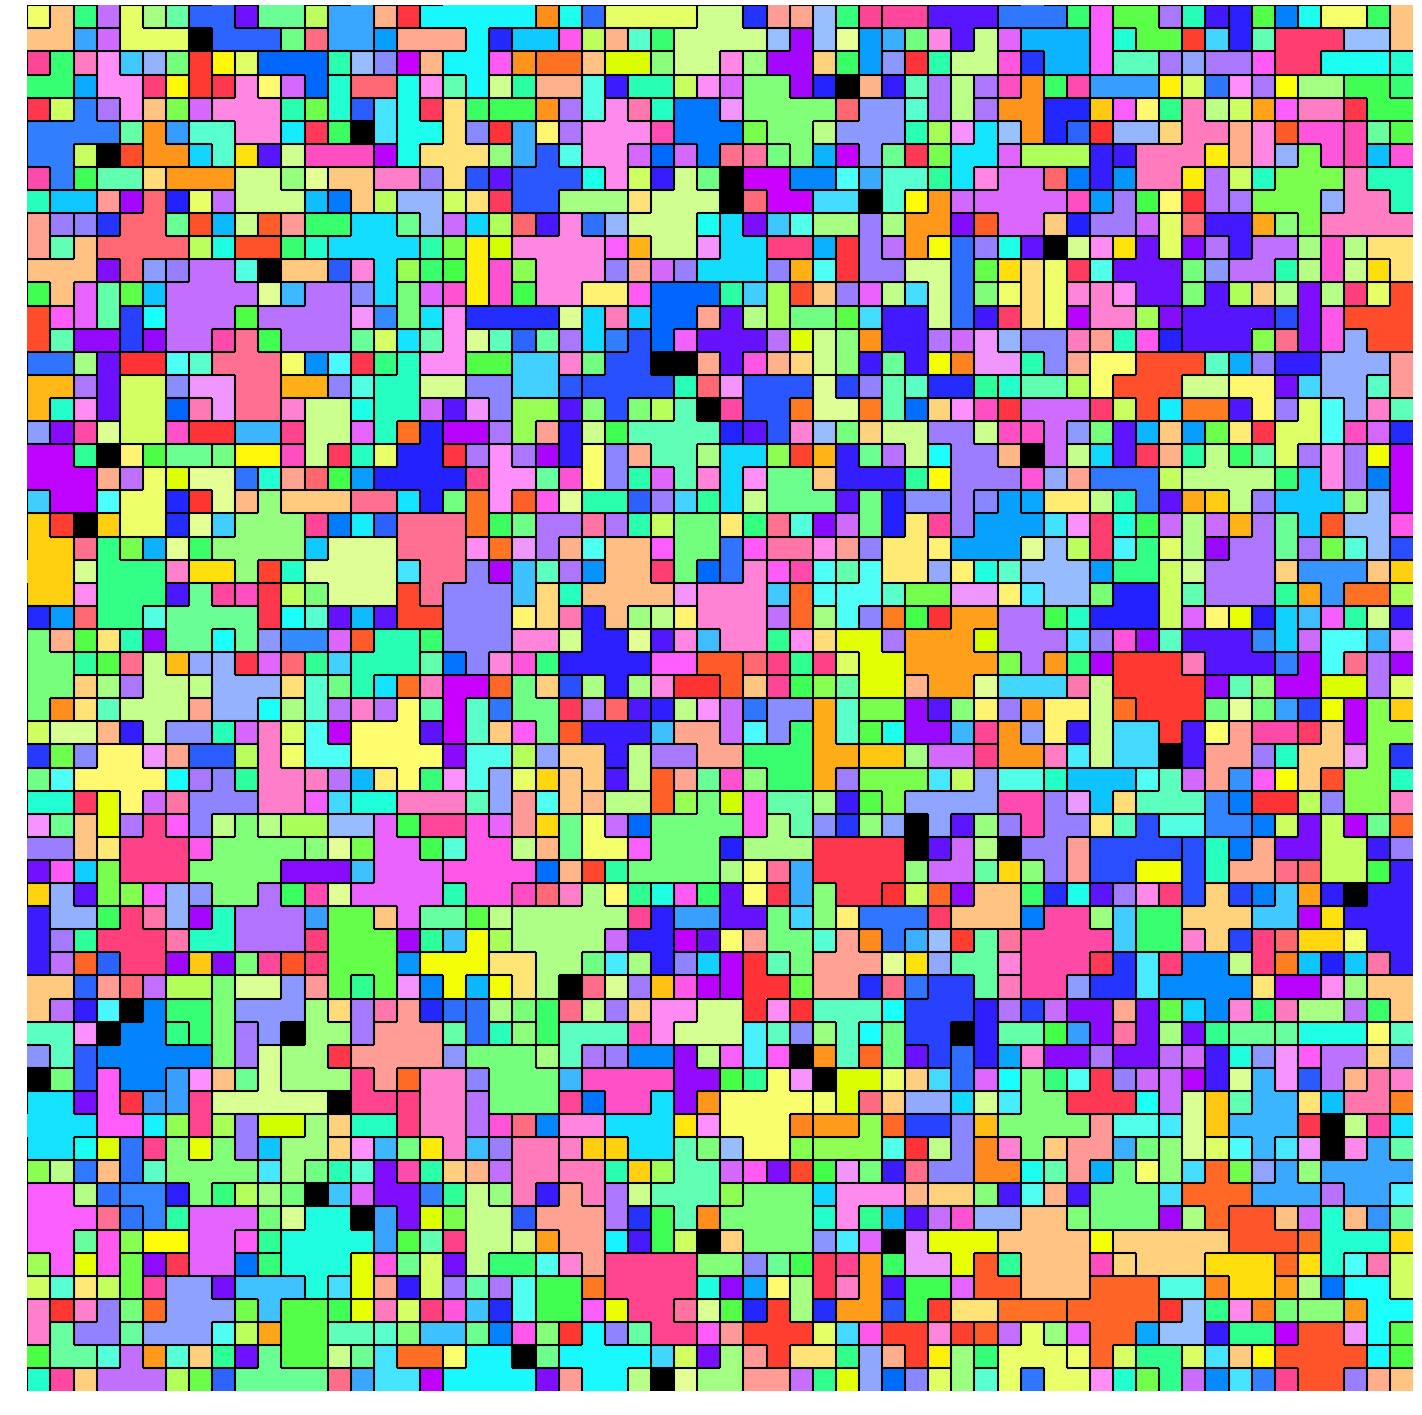
\includegraphics[width=\columnwidth]{seed=1001+title=channel_viz+treat=wave-small__mut-a_low+update=50000+_data_hathash_hash=38f284fb779ed3f5+_script_fullcat_hash=474b4115ecde8750+_source_hash=d53f428-clean+ext=}
\end{subfigure}
\begin{subfigure}[b]{0.45\columnwidth}
  \centering
  Large Resource Wave\\~\\
  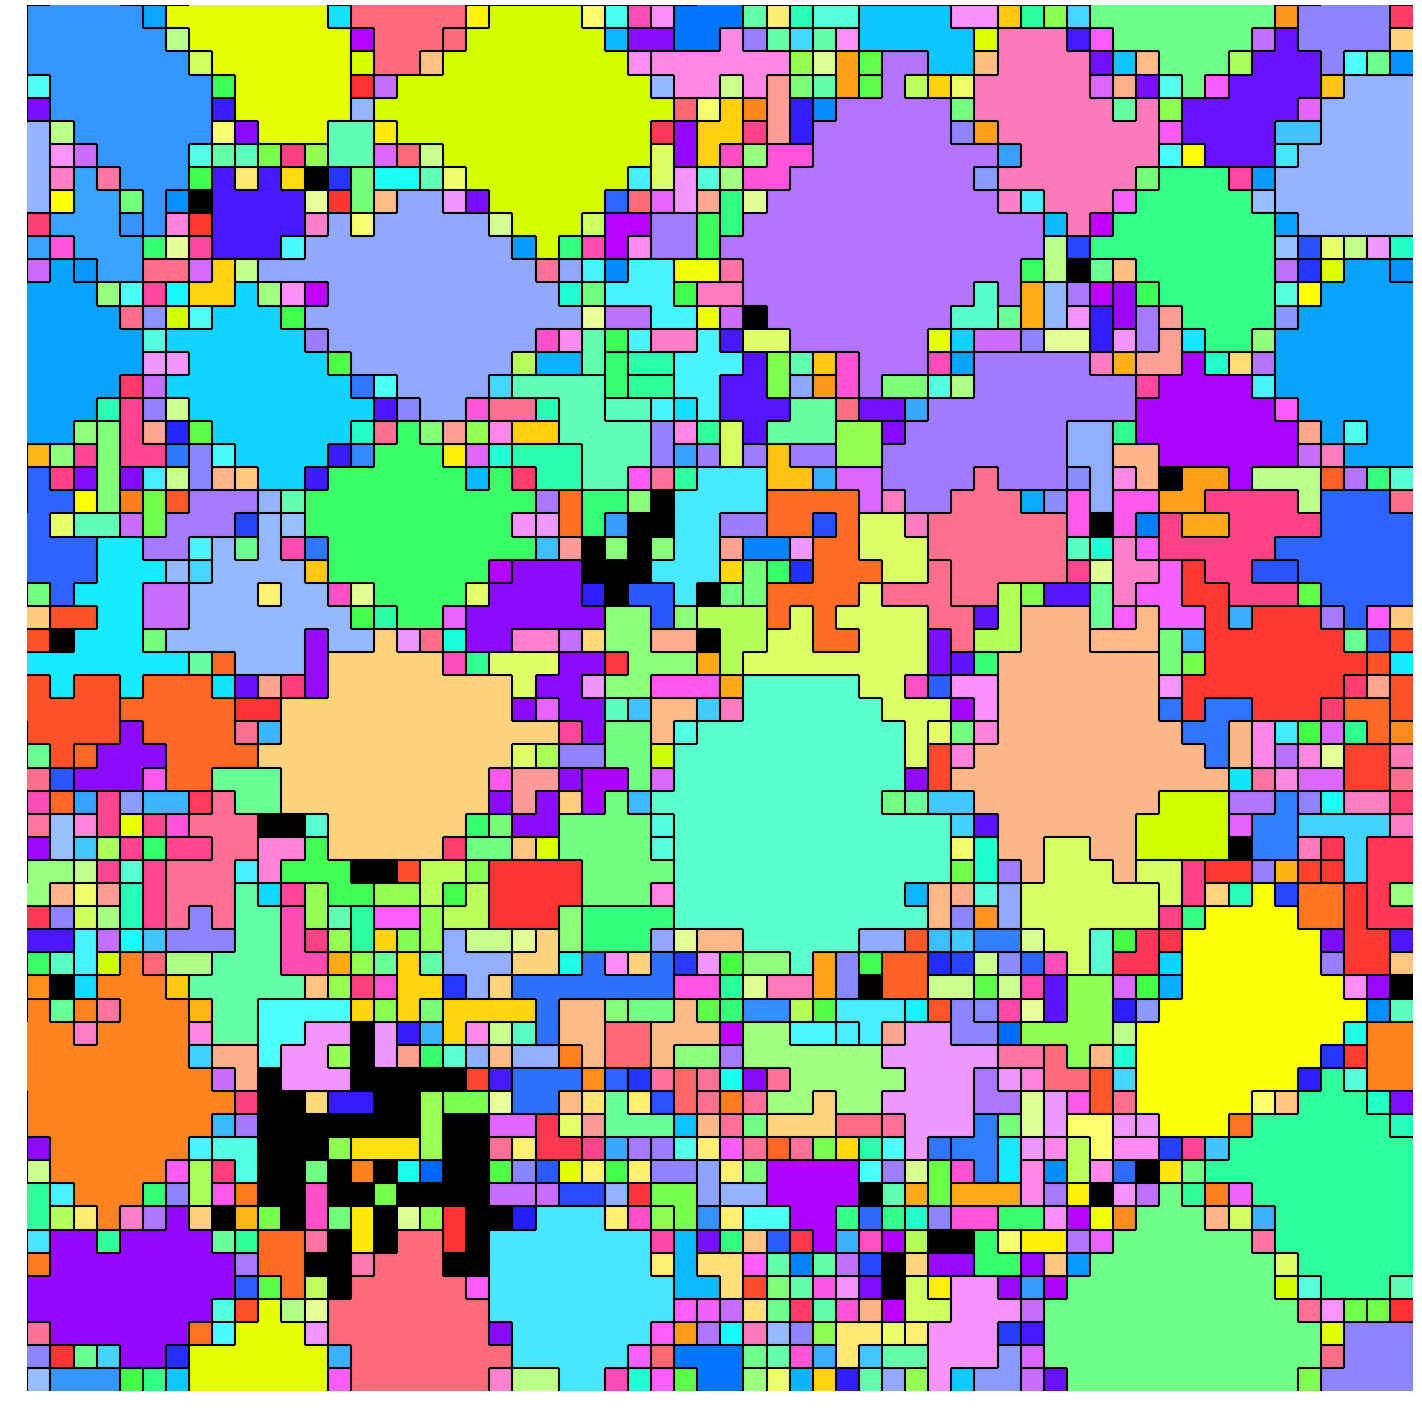
\includegraphics[width=\columnwidth]{seed=1001+title=channel_viz+treat=wave-big__mut-a_low+update=50000+_data_hathash_hash=33ac6f19e90e7ab9+_script_fullcat_hash=474b4115ecde8750+_source_hash=d53f428-clean+ext=}
\end{subfigure}

\rotatebox{90}{~~~~~~~Mutational Load 2}
\begin{subfigure}[b]{0.45\columnwidth}
  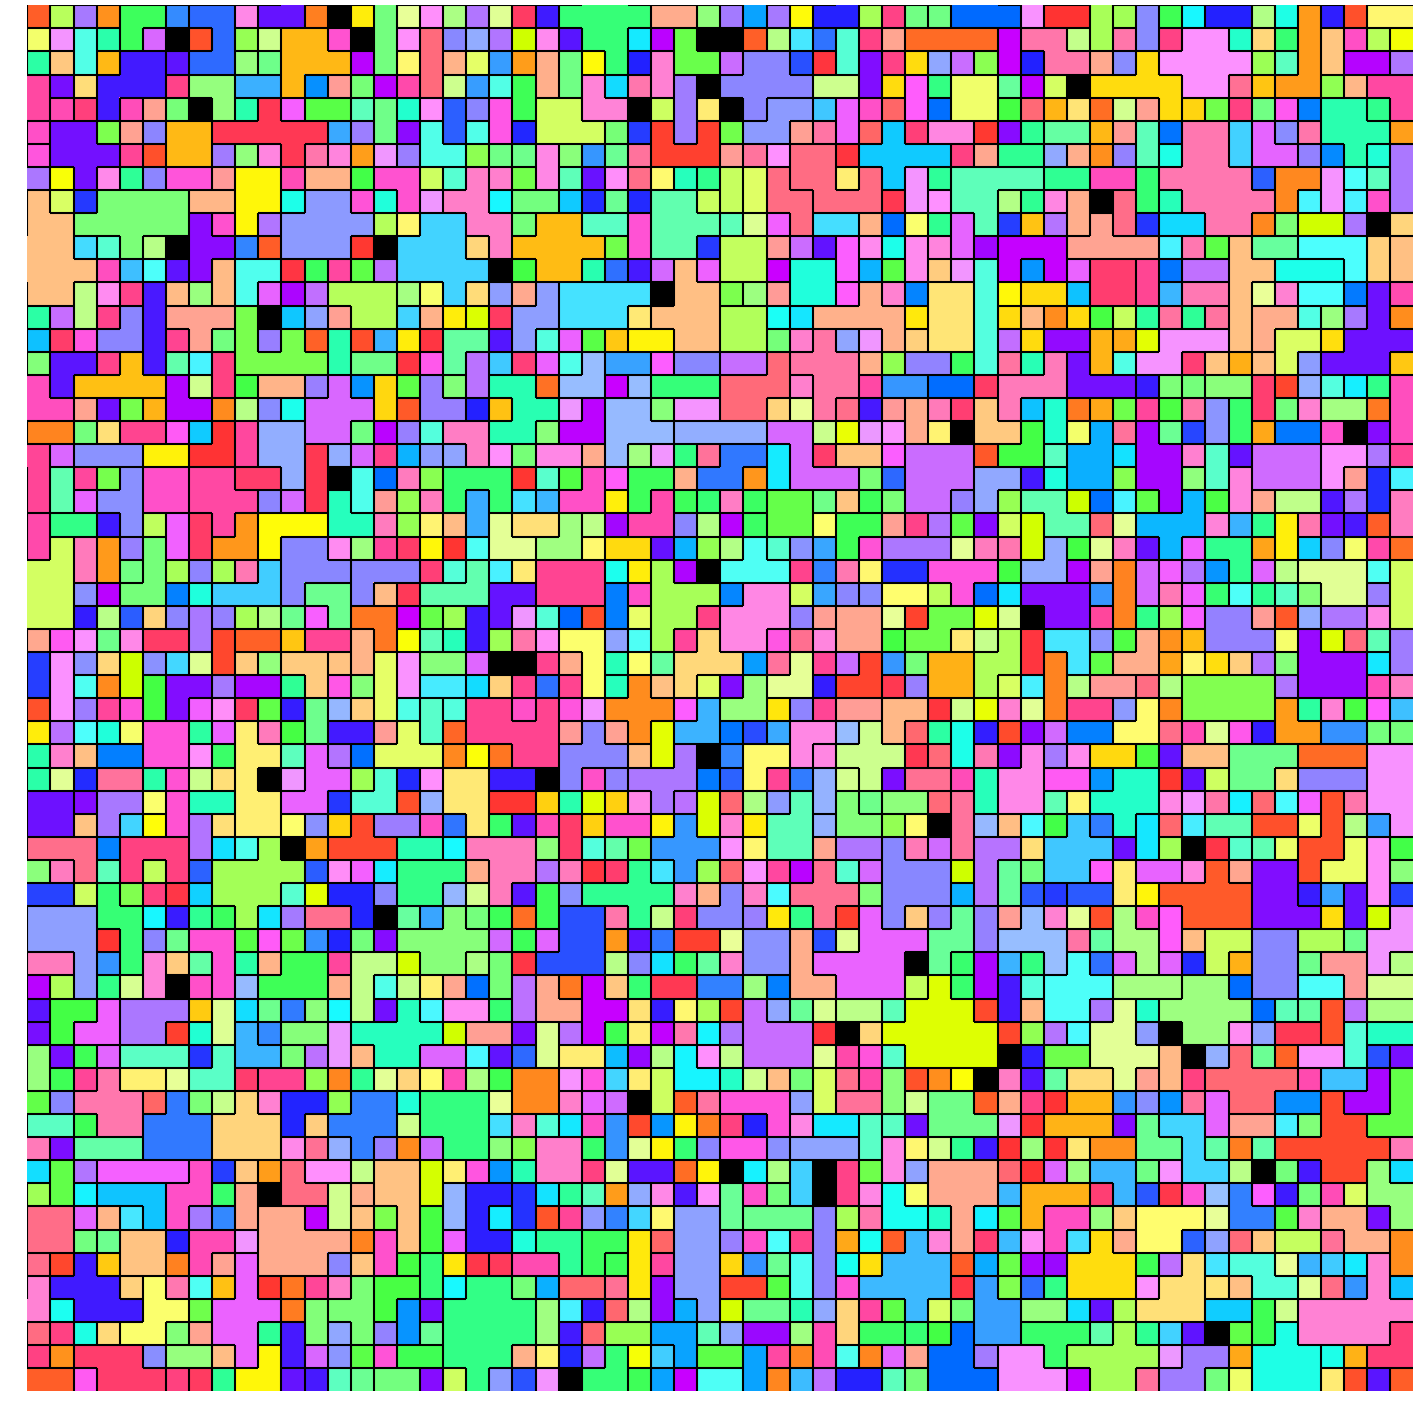
\includegraphics[width=\columnwidth]{seed=1001+title=channel_viz+treat=wave-small__mut-b_medlow+update=50000+_data_hathash_hash=0c0190afbbcd9acb+_script_fullcat_hash=474b4115ecde8750+_source_hash=d53f428-clean+ext=}
\end{subfigure}
\begin{subfigure}[b]{0.45\columnwidth}
  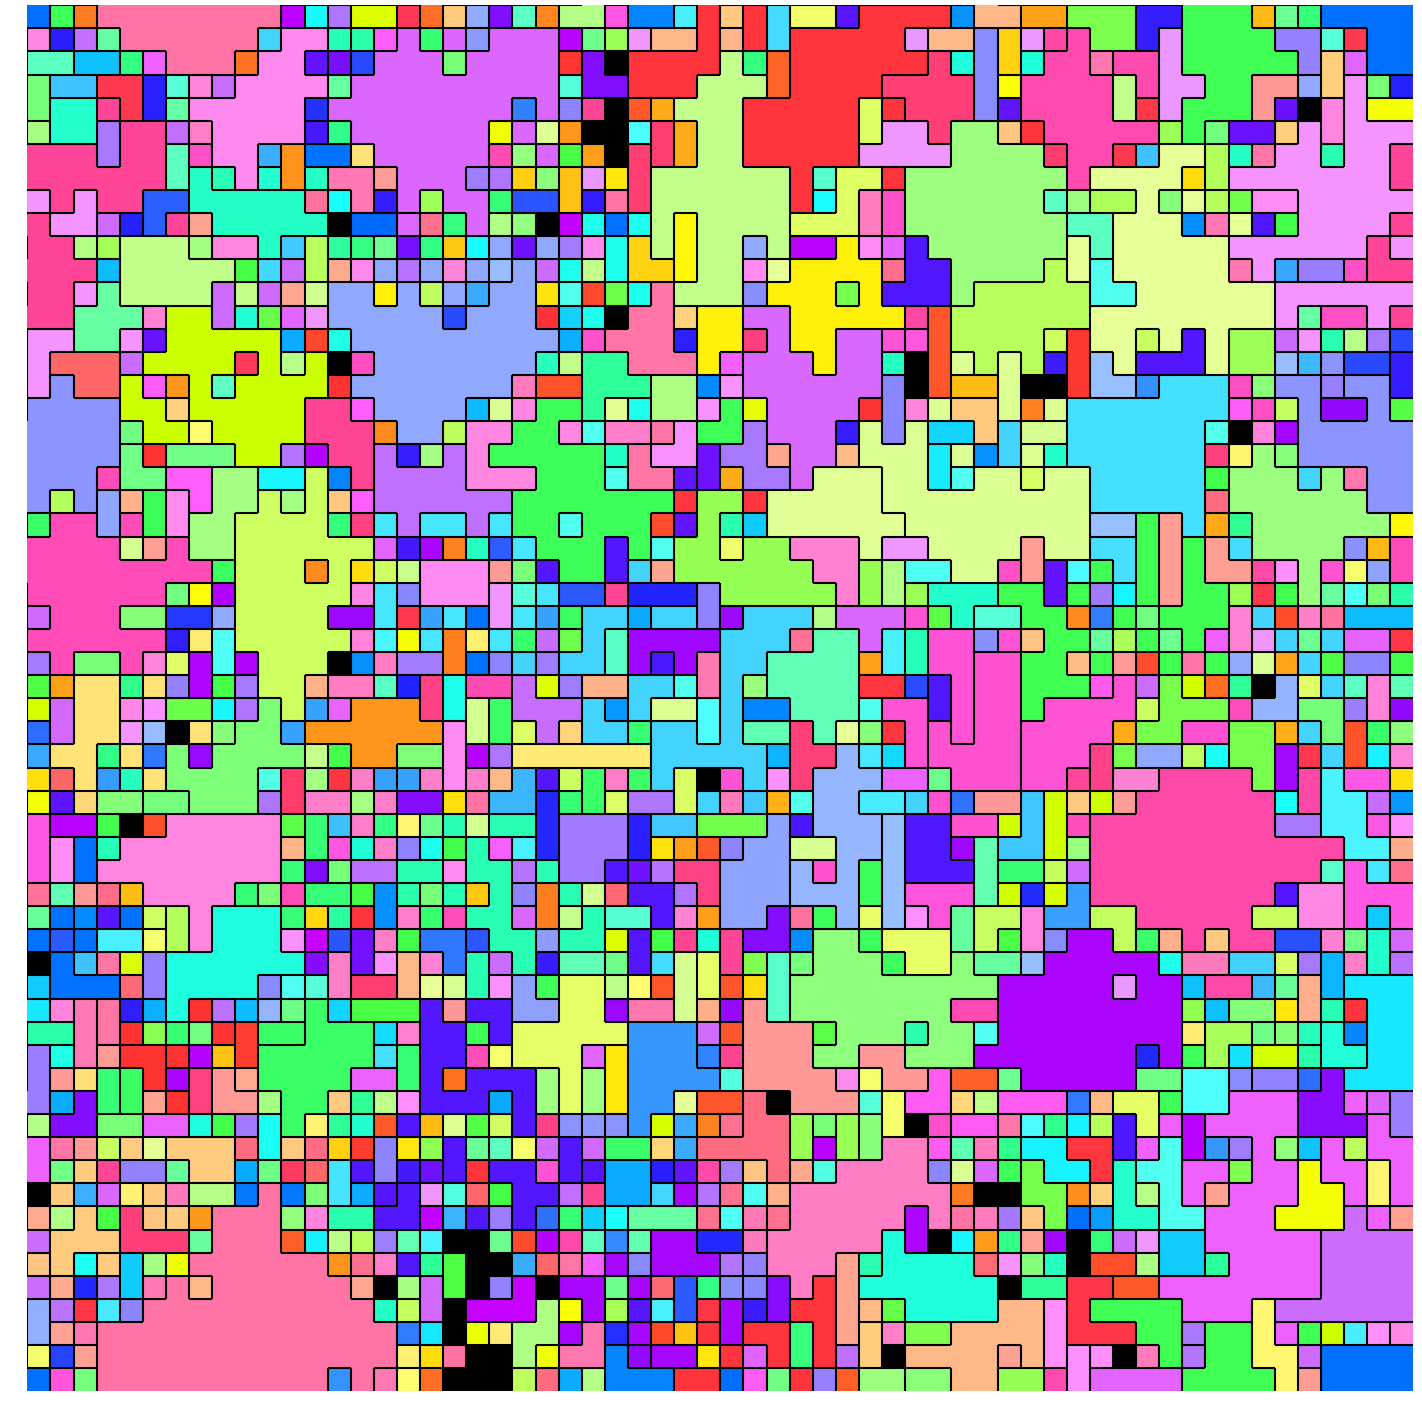
\includegraphics[width=\columnwidth]{seed=1001+title=channel_viz+treat=wave-big__mut-b_medlow+update=50000+_data_hathash_hash=50427fb0ffaf976a+_script_fullcat_hash=474b4115ecde8750+_source_hash=d53f428-clean+ext=}
\end{subfigure}

\rotatebox{90}{~~~~~~~Mutational Load 3}
\begin{subfigure}[b]{0.45\columnwidth}
  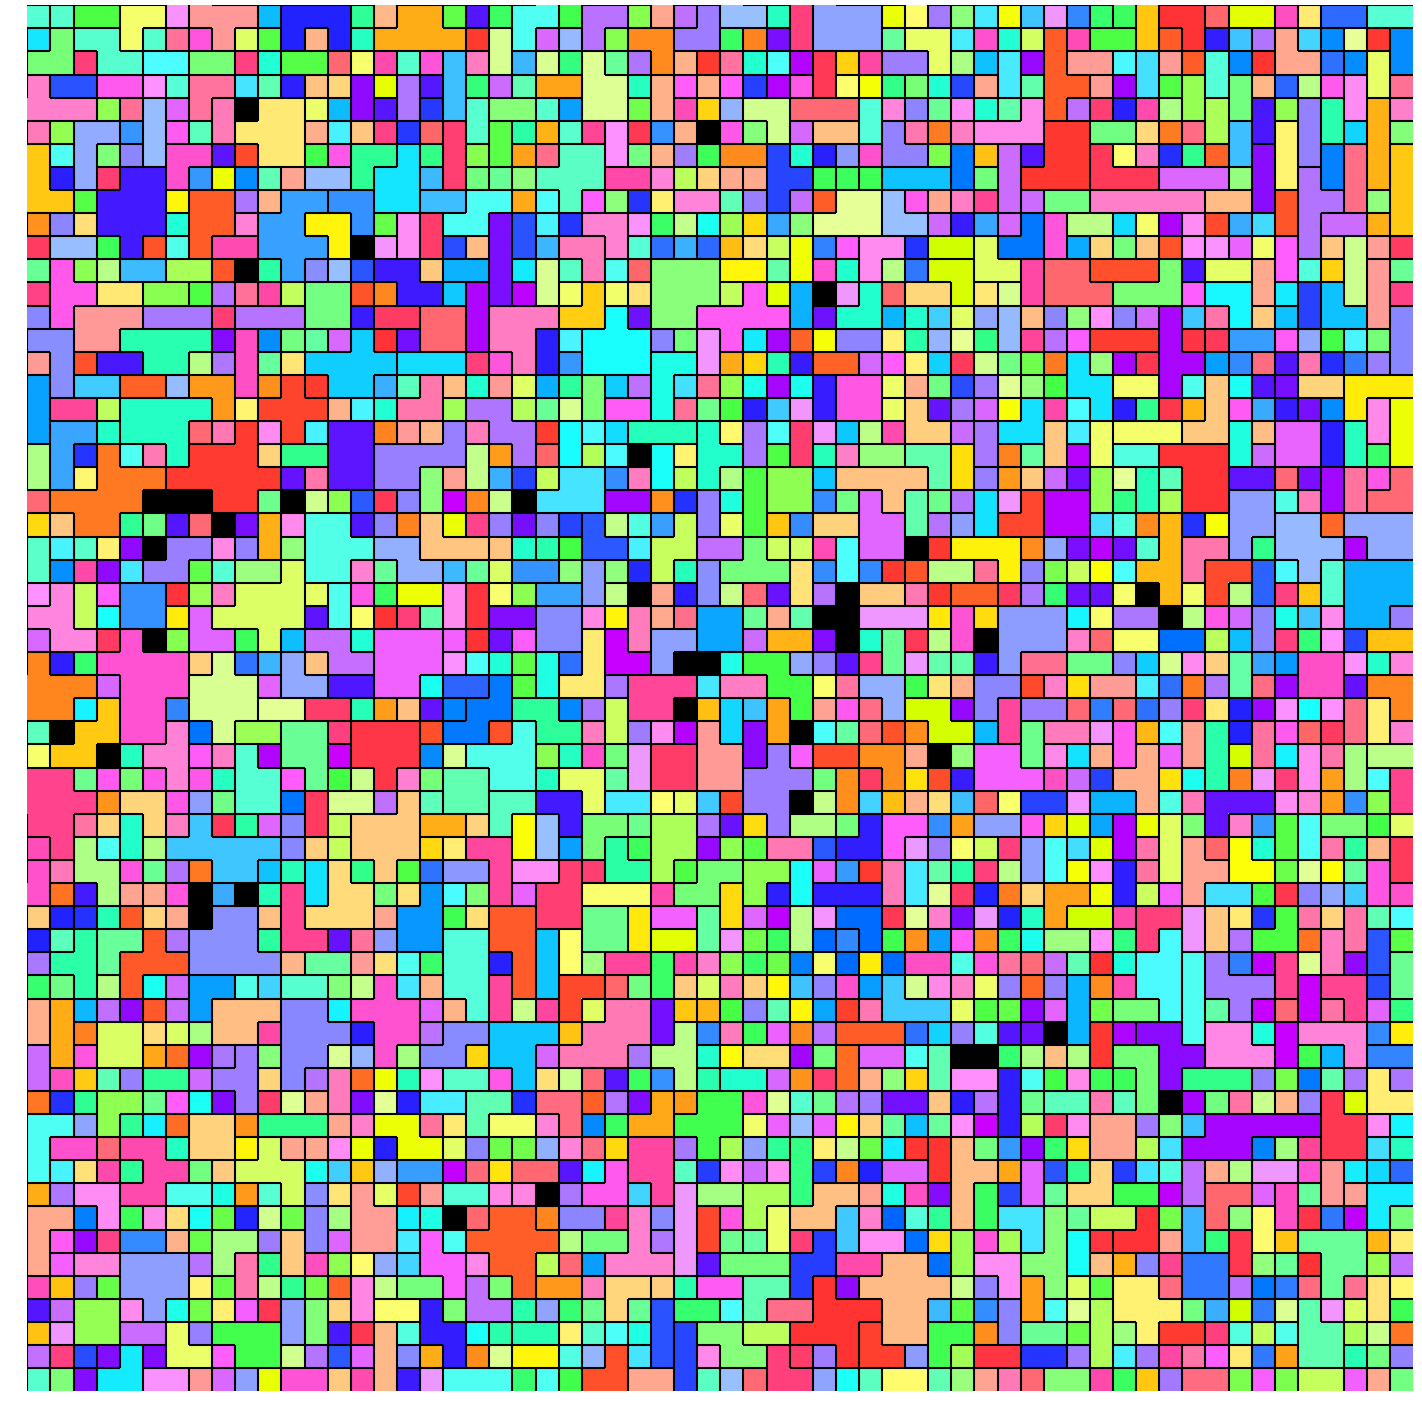
\includegraphics[width=\columnwidth]{seed=1001+title=channel_viz+treat=wave-small__mut-c_medhigh+update=50000+_data_hathash_hash=153e2f8791347e2b+_script_fullcat_hash=474b4115ecde8750+_source_hash=d53f428-clean+ext=}
\end{subfigure}
\begin{subfigure}[b]{0.45\columnwidth}
  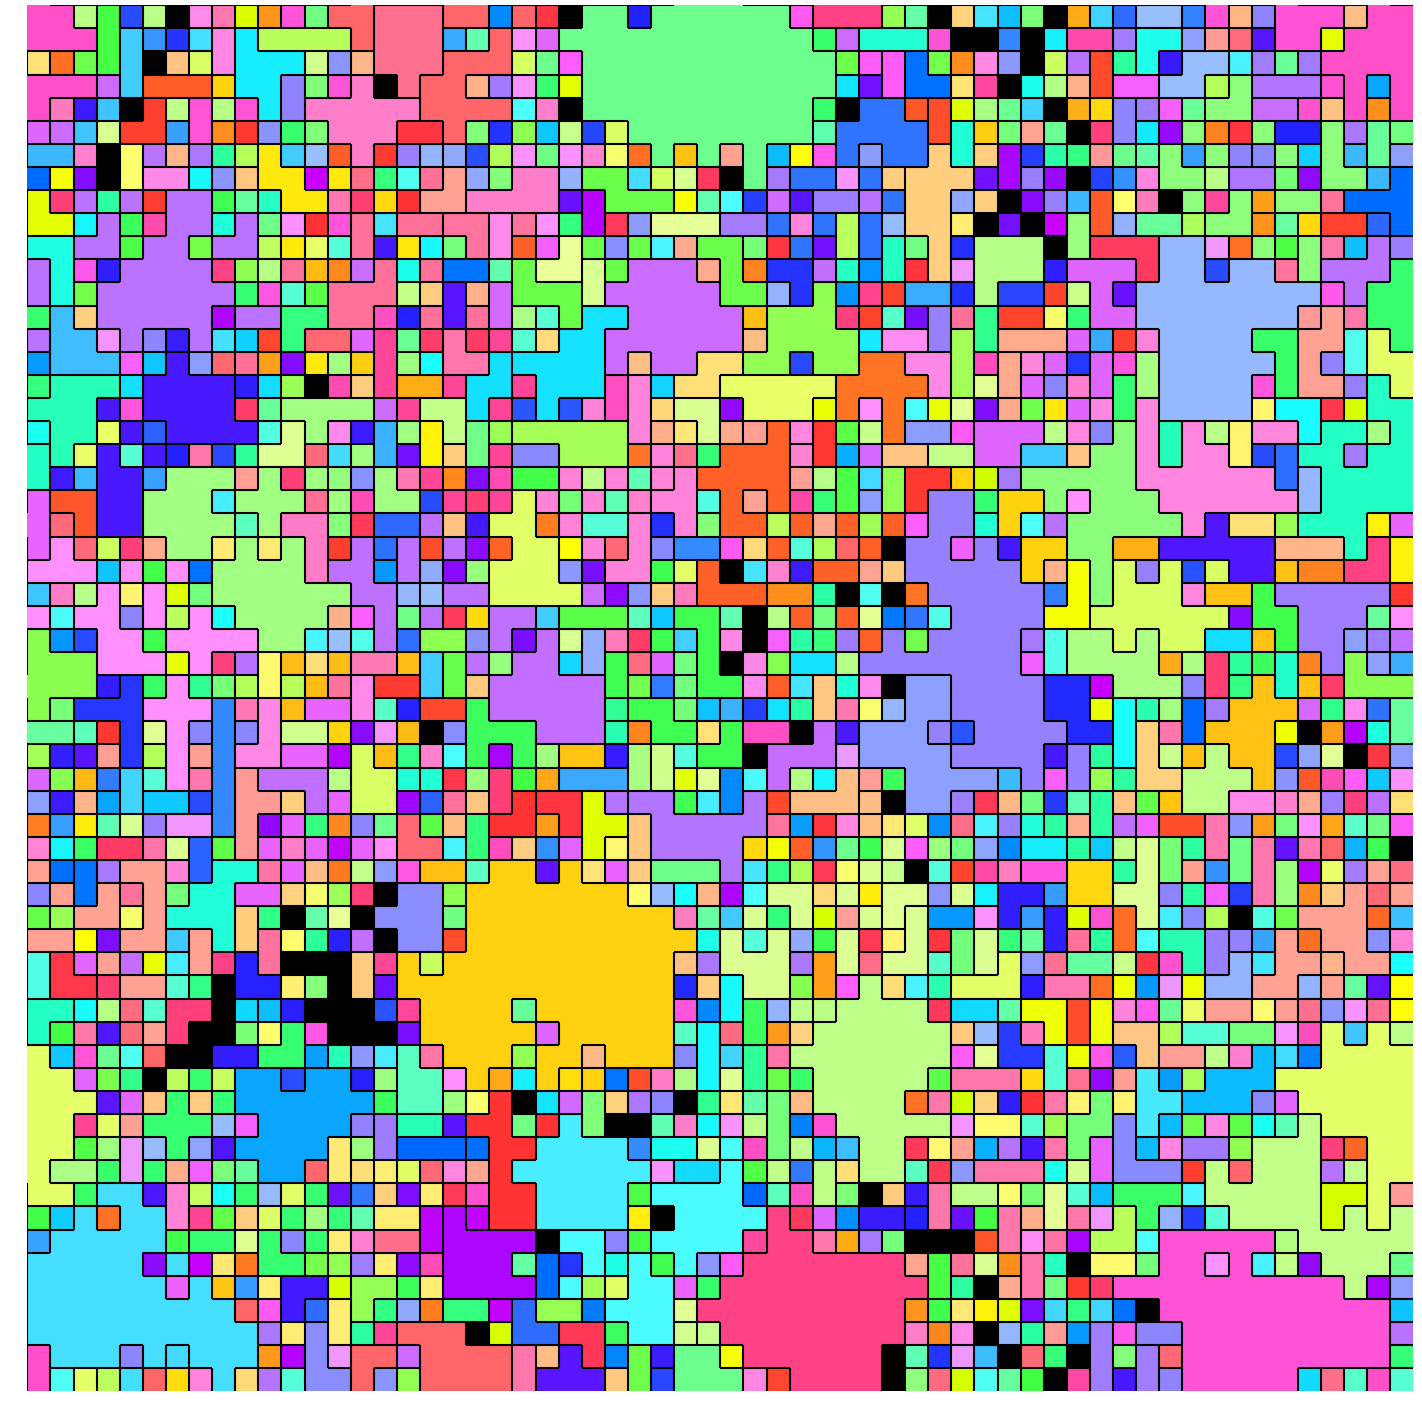
\includegraphics[width=\columnwidth]{seed=1001+title=channel_viz+treat=wave-big__mut-c_medhigh+update=50000+_data_hathash_hash=3bc8464cdb13317c+_script_fullcat_hash=474b4115ecde8750+_source_hash=d53f428-clean+ext=}
\end{subfigure}

\rotatebox{90}{~~~~~~~Mutational Load 4}
\begin{subfigure}[b]{0.45\columnwidth}
  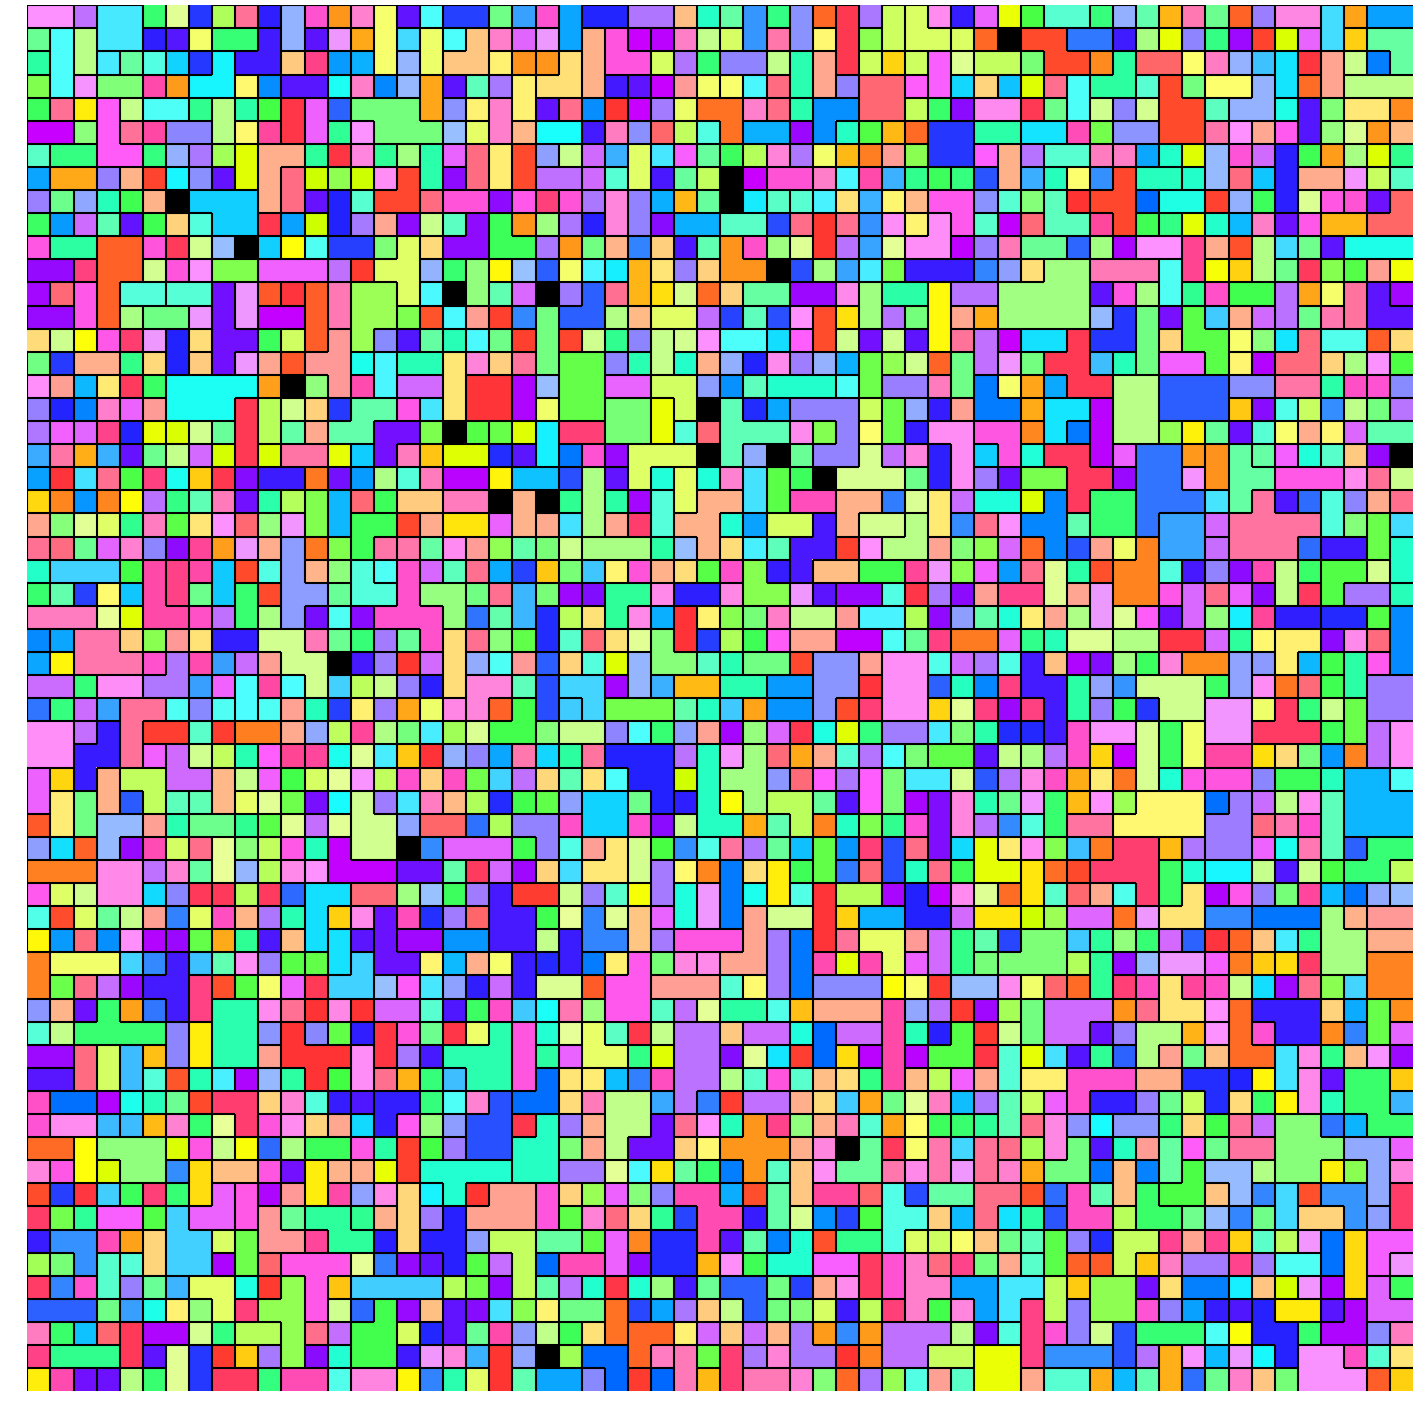
\includegraphics[width=\columnwidth]{seed=1001+title=channel_viz+treat=wave-small__mut-d_high+update=50000+_data_hathash_hash=700947e5ae80d046+_script_fullcat_hash=474b4115ecde8750+_source_hash=d53f428-clean+ext=}
\end{subfigure}
\begin{subfigure}[b]{0.45\columnwidth}
  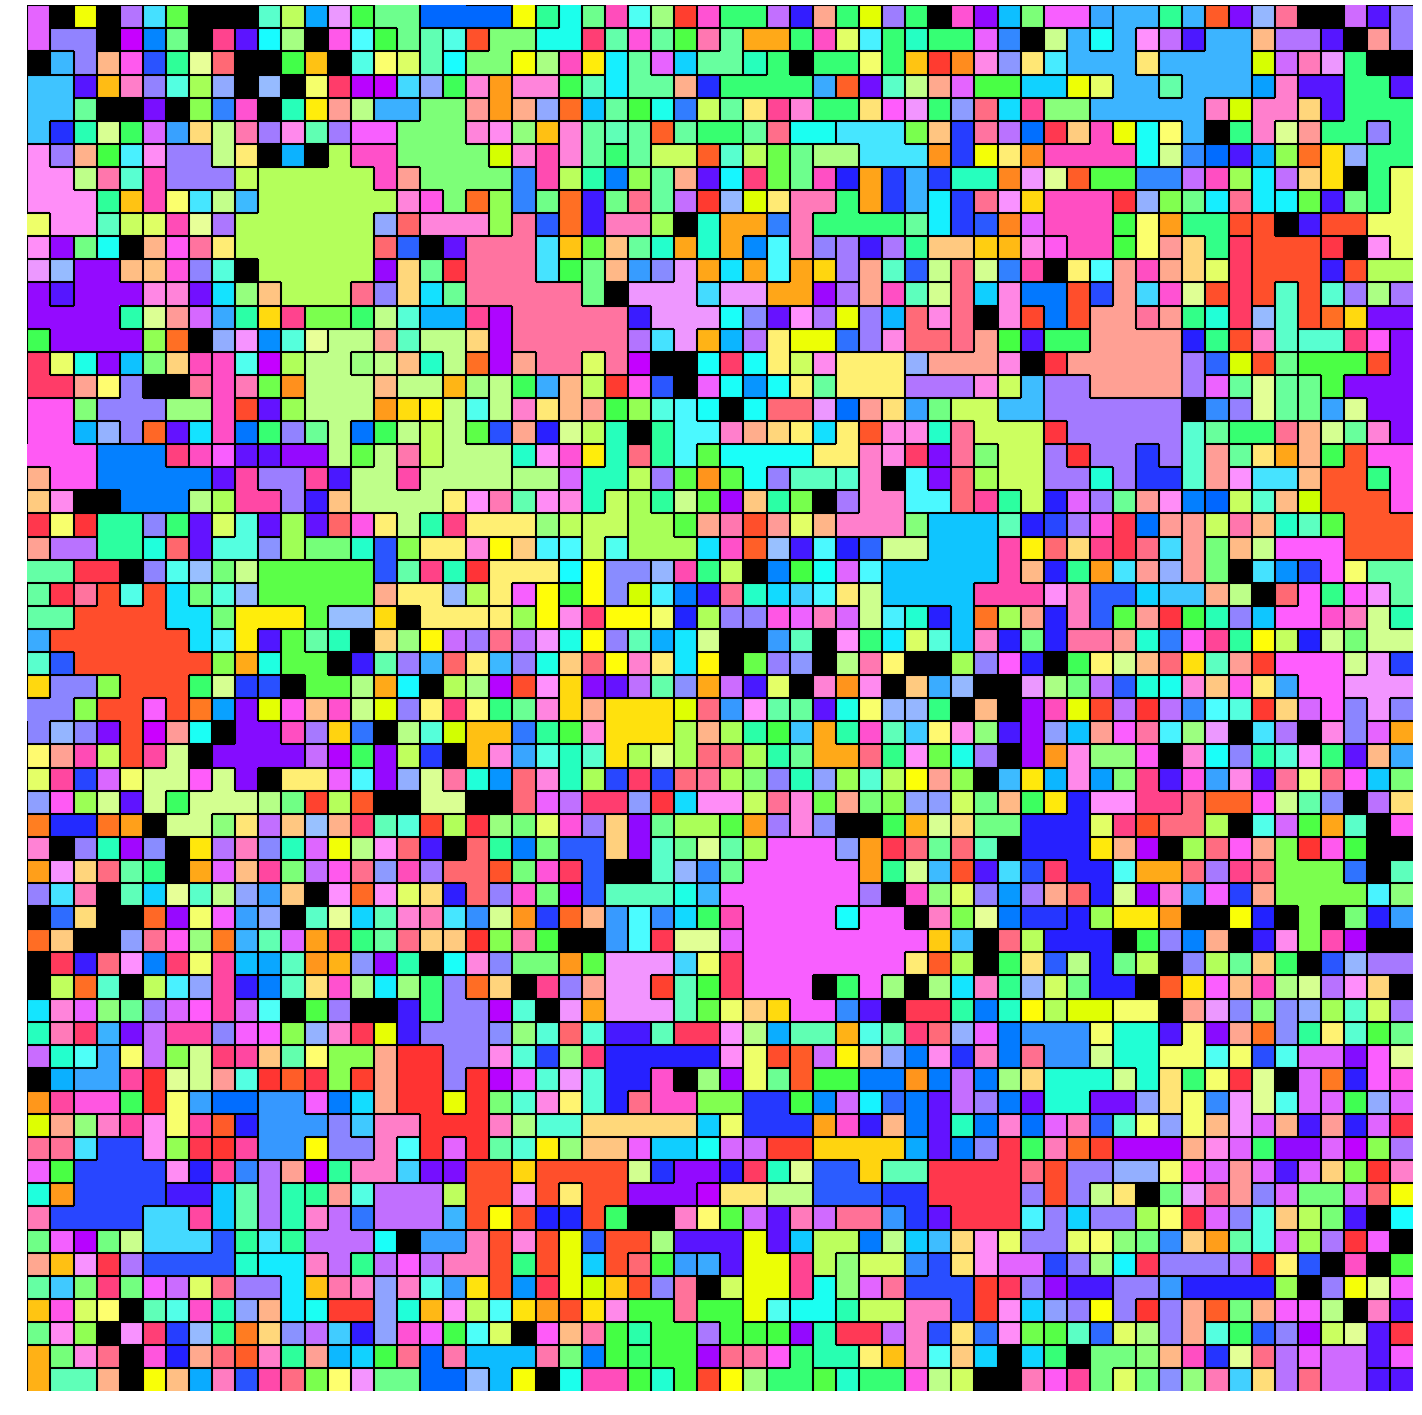
\includegraphics[width=\columnwidth]{seed=1001+title=channel_viz+treat=wave-big__mut-d_high+update=50000+_data_hathash_hash=e7071e390f076a00+_script_fullcat_hash=474b4115ecde8750+_source_hash=d53f428-clean+ext=}
\end{subfigure}

\rotatebox{90}{~~~~~~~Mutational Load 5}
\begin{subfigure}[b]{0.45\columnwidth}
  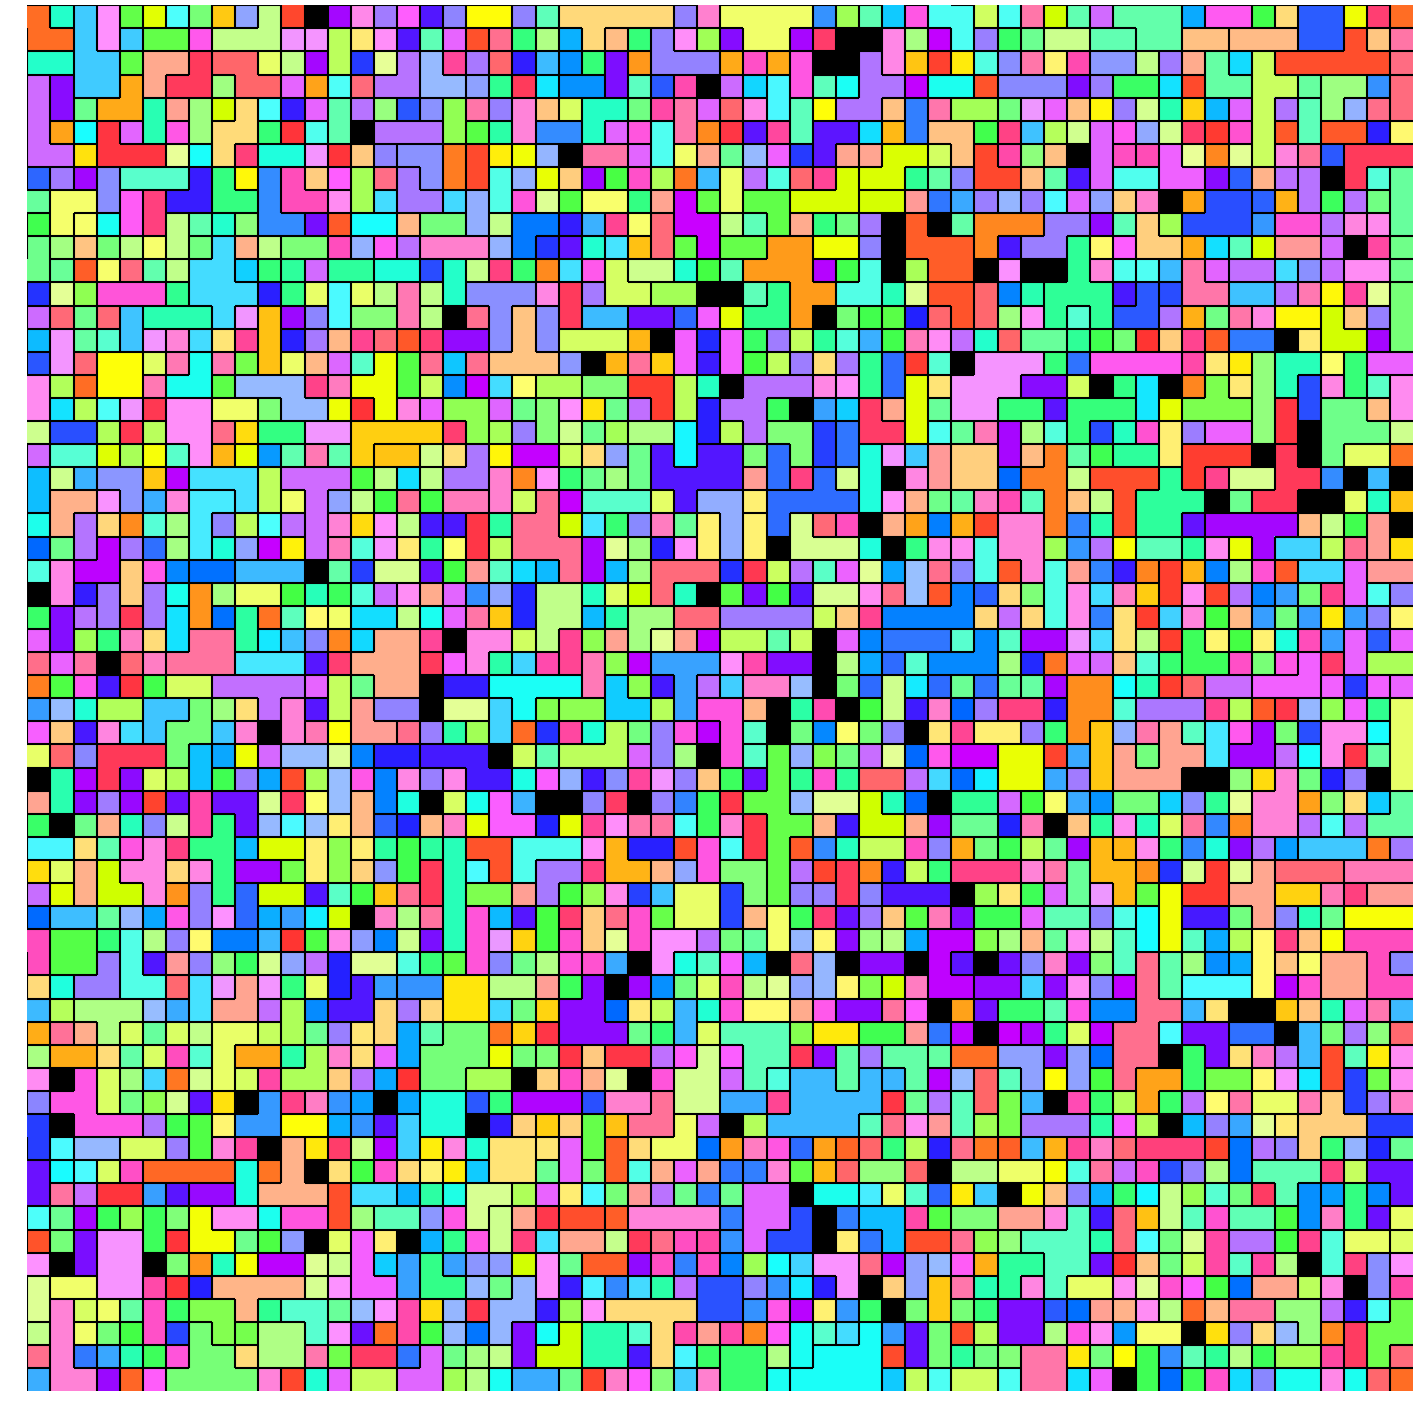
\includegraphics[width=\columnwidth]{seed=1001+title=channel_viz+treat=wave-small__mut-e_extreme+update=50000+_data_hathash_hash=70d59bcccb7f3ca6+_script_fullcat_hash=474b4115ecde8750+_source_hash=d53f428-clean+ext=}
\end{subfigure}
\begin{subfigure}[b]{0.45\columnwidth}
  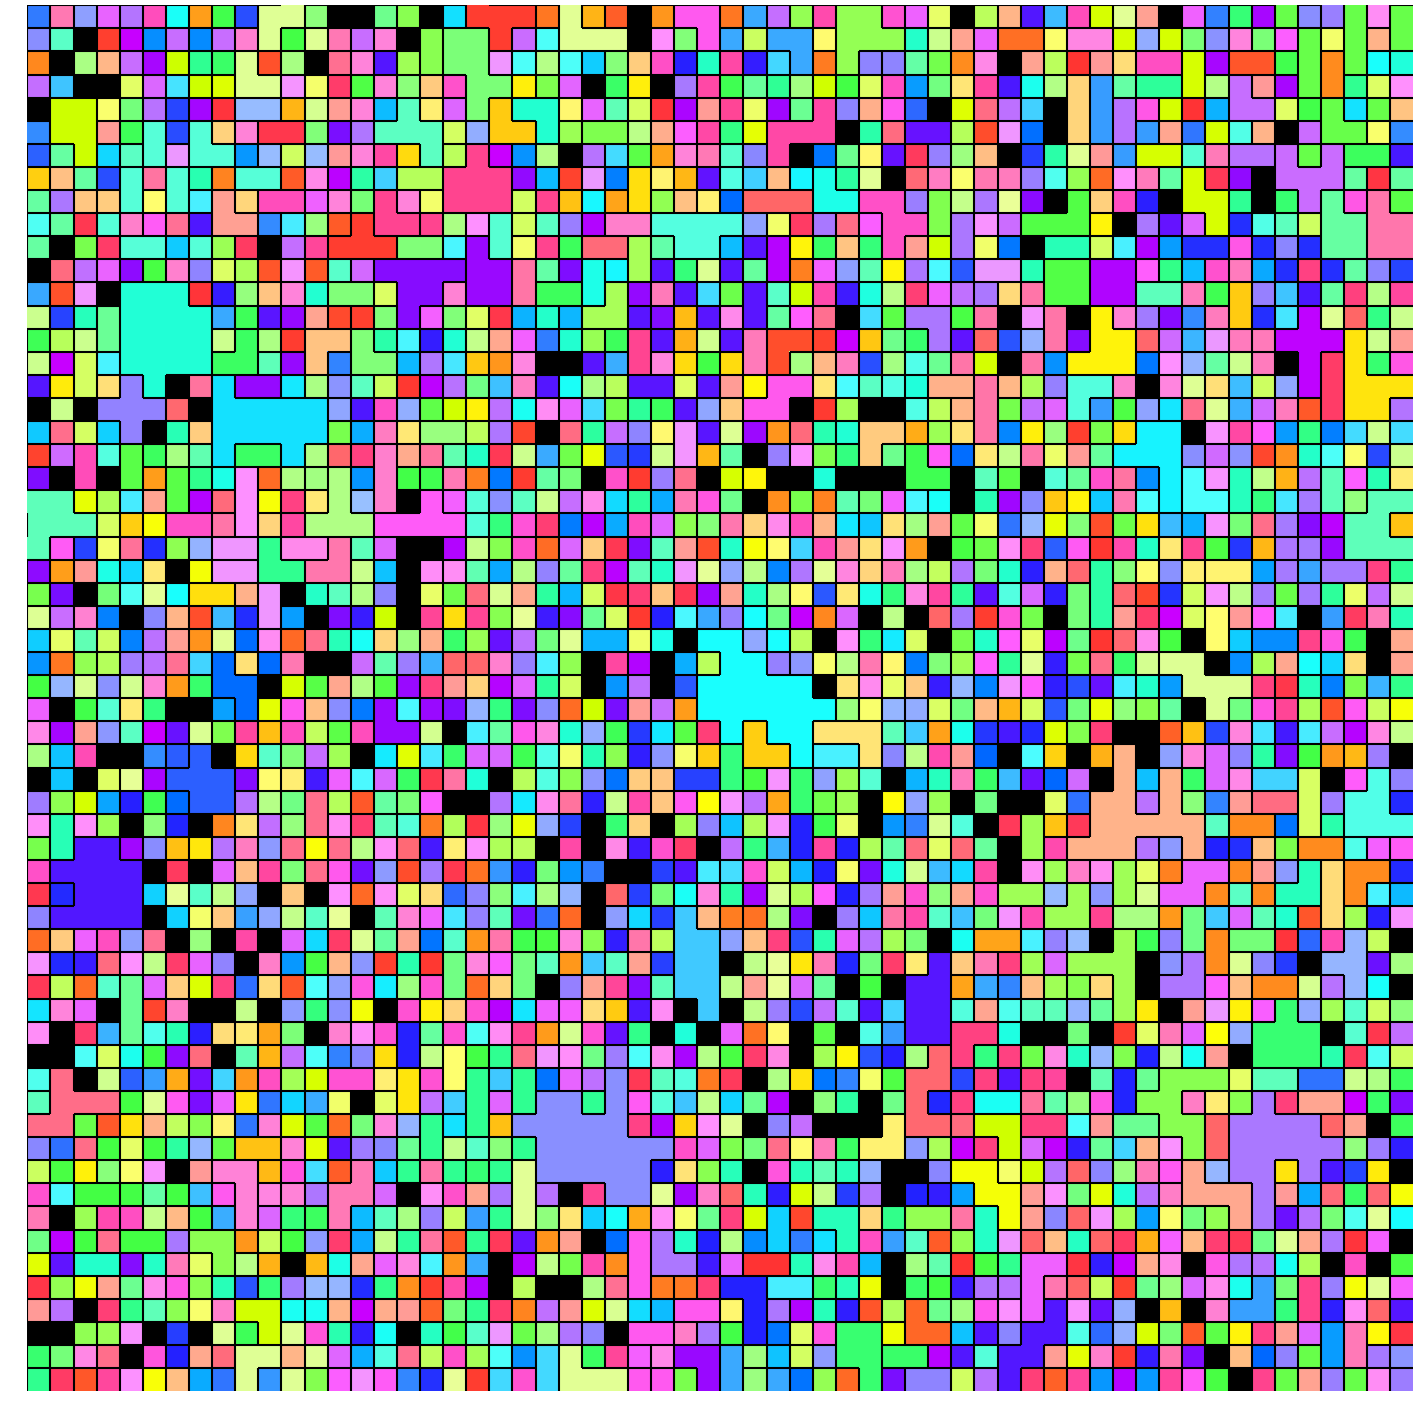
\includegraphics[width=\columnwidth]{seed=1001+title=channel_viz+treat=wave-big__mut-e_extreme+update=50000+_data_hathash_hash=6532b779898a7959+_script_fullcat_hash=474b4115ecde8750+_source_hash=d53f428-clean+ext=}
\end{subfigure}
\caption{
Representative same-channel signaling network end states for runs of each treatment.
A single cell-like organism occupies each grid tile except for black tiles, which are empty.
Channel IDs are coded by color.
Same-channel groups appear as uniformly-colored clumps, bounded by a black border.
}
\label{fig:outcome_grids}
\end{center}
\end{figure}


\begin{figure}[!htbp]
\begin{center}
\begin{subfigure}[b]{0.49\columnwidth}
  
\includegraphics[width=\columnwidth]{source_hash=de48c04-dirty_emp_hash=1c7cb544-clean_title=channel_viz+treat=resource-wave__channelsense-yes__nlev-two+seed=1+update=0}
  \caption{Update 0; gen. 0}
  \label{fig:TODO}
\end{subfigure}
\begin{subfigure}[b]{0.49\columnwidth}
  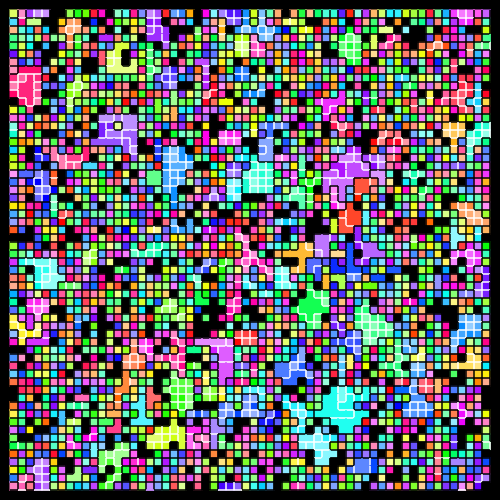
\includegraphics[width=\columnwidth]{source_hash=de48c04-dirty_emp_hash=1c7cb544-clean_title=channel_viz+treat=resource-wave__channelsense-yes__nlev-two+seed=1+update=2500}
  \caption{Update 2.5k; gen. TODO}
  \label{fig:TODO}
\end{subfigure}
\begin{subfigure}[b]{0.49\columnwidth}
  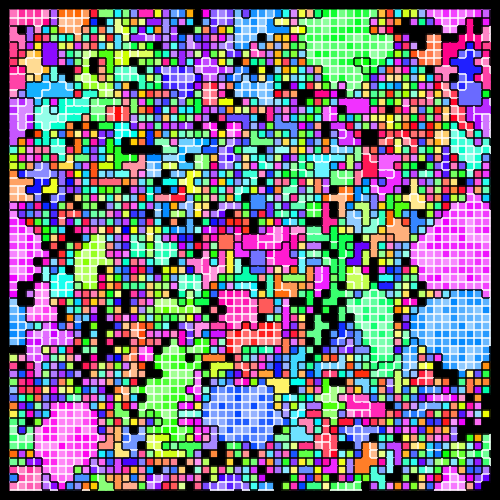
\includegraphics[width=\columnwidth]{source_hash=de48c04-dirty_emp_hash=1c7cb544-clean_title=channel_viz+treat=resource-wave__channelsense-yes__nlev-two+seed=1+update=5000}
  \caption{Update 5k; gen. TODO}
  \label{fig:TODO}
\end{subfigure}
\begin{subfigure}[b]{0.49\columnwidth}
  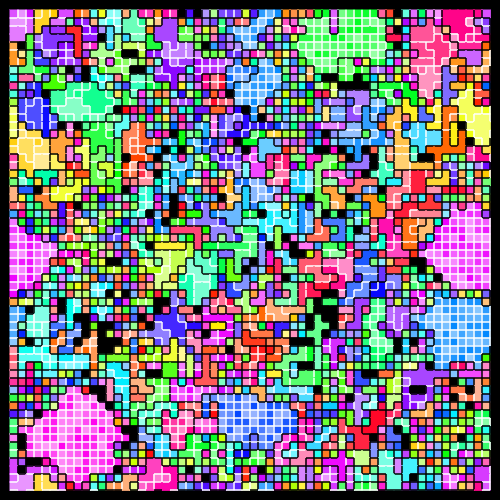
\includegraphics[width=\columnwidth]{source_hash=de48c04-dirty_emp_hash=1c7cb544-clean_title=channel_viz+treat=resource-wave__channelsense-yes__nlev-two+seed=1+update=7500}
  \caption{Update 7.5k; gen. TODO}
  \label{fig:TODO}
\end{subfigure}
\begin{subfigure}[b]{0.49\columnwidth}
  
\includegraphics[width=\columnwidth]{source_hash=de48c04-dirty_emp_hash=1c7cb544-clean_title=channel_viz+treat=resource-wave__channelsense-yes__nlev-two+seed=1+update=10000}
  \caption{Update 10k; gen. TODO}
  \label{fig:TODO}
\end{subfigure}
\begin{subfigure}[b]{0.49\columnwidth}
  
\includegraphics[width=\columnwidth]{source_hash=de48c04-dirty_emp_hash=1c7cb544-clean_title=channel_viz+treat=resource-wave__channelsense-yes__nlev-two+seed=1+update=20000}
  \caption{Update 20k; gen. TODO}
  \label{fig:TODO}
\end{subfigure}
\begin{subfigure}[b]{0.49\columnwidth}
  
\includegraphics[width=\columnwidth]{source_hash=de48c04-dirty_emp_hash=1c7cb544-clean_title=channel_viz+treat=resource-wave__channelsense-yes__nlev-two+seed=1+update=30000}
  \caption{Update 30k; gen. TODO}
  \label{fig:TODO}
\end{subfigure}
\begin{subfigure}[b]{0.49\columnwidth}
  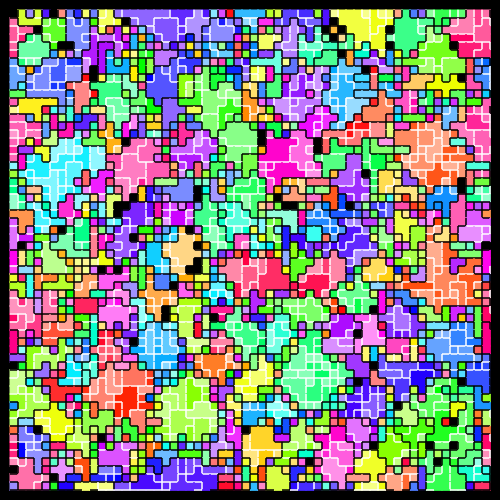
\includegraphics[width=\columnwidth]{source_hash=de48c04-dirty_emp_hash=1c7cb544-clean_title=channel_viz+treat=resource-wave__channelsense-yes__nlev-two+seed=1+update=50000}
  \caption{Update 50k; gen. TODO}
  \label{fig:TODO}
\end{subfigure}
\caption{
Progression of of same-channel level-zero and level-one signaling networks states in an evolutionary run.
In the "Channel Viewer", low-level groups are coded by color saturation (divided by white lines) and high-level groups are coded by color hue (divided by black lines).
Black grid tiles represent empty channel ID.
}
\label{fig:grid_progression}
\end{center}
\end{figure}


\begin{figure}[!htbp]
\begin{center}

\begin{subfigure}[b]{0.5\columnwidth}
  \includegraphics[width=\columnwidth]{img/champion_res_pool1_vs_champion_damage_suicide0}
  \caption{
  Correlation plot of dominant genotype $P_0$ and dominant genotype $M_{c}$.
  }
  \label{fig:champion_res_pool1_vs_champion_damage_suicide0}
\end{subfigure}%
\begin{subfigure}[b]{0.5\columnwidth}
  \includegraphics[width=\columnwidth]{img/champion_res_pool2_vs_champion_damage_suicide0}
  \caption{
  Correlation plot of dominant genotype $P_1$ and dominant genotype $M_{c}$.
  }
  \label{fig:champion_res_pool2_vs_champion_damage_suicide0}
\end{subfigure}

\caption{
Plots of dominant resource caching strategies and dominant apoptosis strategies.
A bootstrapped 95\% confidence interval for the fit is shaded.
}
\label{fig:damage_suicide}
\end{center}
\end{figure}


\input{fig/net_reproduction.tex}

\begin{figure}[!htbp]
\begin{center}

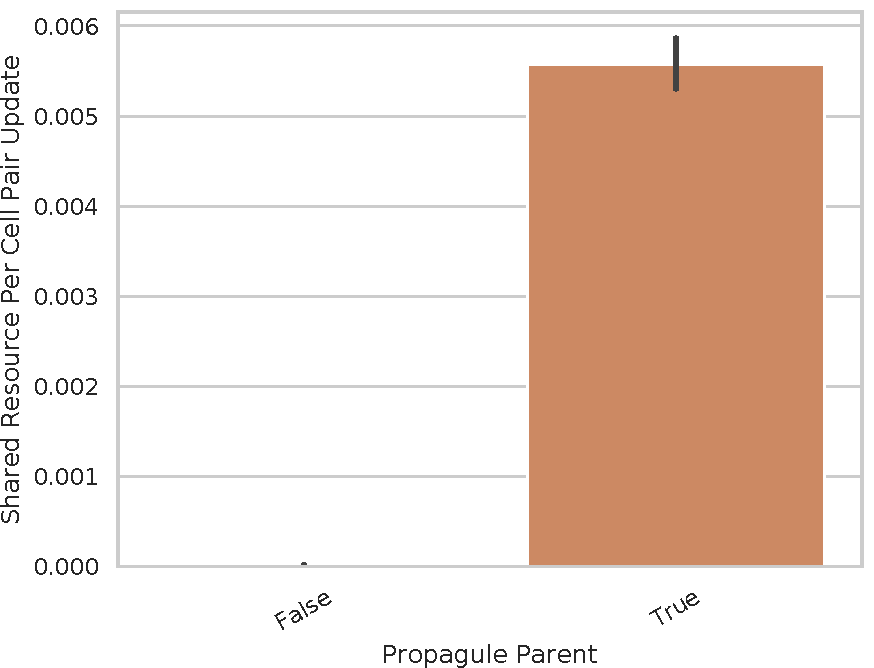
\includegraphics[width=\columnwidth]{script_hash=TODO_source_hash=TODO_emp_hash=TODO_treat=resource-wave__channelsense-yes__nlev-two+seed=1018+title=propagule_parent_resource_contributed}
\caption{
Replicate with seed 1018 from standard treatment.
}
\label{fig:endowment}
\end{center}
\end{figure}


Cell-, zeroth-, and first-level individuals were all observed at the conclusion of different runs of our evolutionary simulation (mean generation 22,016; $s=3,119$).
The criteria used to discern these outcomes are described below.
Figure \ref{fig:outcome_grids} shows the level-zero and level-one signaling networks at the end of runs where cell-, zeroth-, and first-level individuality evolved, respectively.
Figure \ref{fig:grid_progression} shows a time series of signaling network snapshots in an evolutionary run where first-level individuality evolved.
Cell-level individuals appear to form with comparatively large level-zero signaling networks that are arranged into amorphous level-one signaling networks.
Zeroth-level individuals appear to form elongated cigar-shaped level-one amalgamations of diverse level-zero networks.
First-level individuals appear to form highly regular diamond-shaped level-one amalgamations of diverse level-zero networks.

Figure \ref{fig:genotypes} describes predominant genotypes observed at the end of our evolutionary simulations.
With a single exception, nearly all evolved genotypes had $A_1$ fixed at or very near $1.0$ (i.e. population mean $A_1 \geq 0.993$).
So, reproduction over cells sharing the same level-one channel was near-universally avoided;
genotypes evolved so that cell-level organisms declined to reproduce when they were located at the interior of level-one same-channel signaling networks.

However, a variety of resource-caching strategies evolved.
Most-abundant genotypes at the end of evolutionary runs included strategies where resource was primarily cached in an organism's individual stockpile (i.e. $P_{c} > P_0, P_1$), strategies where resource was primarily cached in an organism's level-zero signaling network's pool (i.e. $P_0 > P_{c}, P_1$), and strategies where resource was primarily cached in an organism's level-one signaling network's pool (i.e. $P_1 > P_{c}, P_0$).
Among 33 trials, selfish cell-level hoarders dominated at the end of two replicates, level-zero resource-sharing dominated in 16 replicates, and level-one resource sharing dominated in 15 replicates.

Given the near-ubiquitous nature of cooperation with regard to reproductive division of labor at the level-one same-channel signaling network, it was on this basis of resource caching strategy that we drew distinctions between cell-, zeroth-, and first-level individuality.
(The single predominant genotype with $A_1 = 0.91$ had $P_0 = 1.0$, so was not sharing resource on the level-one same-channel resource pool).
% @CAO: I'm not sure where this final parenthetical came from.  I take it this is the single "selfish" individual in the second example above?
% @MAM: Exactly.

Next, we wanted to compare cell-, zeroth-, and first-level individuals to determine which genotype was the most fit in the DISHTINY platform environment.
We ran ecological competitions between the the dominant genotypes from the run with greatest mean $P_{c}$, the run with greatest mean $P_0$, and the run with greatest mean $P_1$.
In 22 out of 191 trials performed fixation was reached by update 1.5 million.  The cell-level individuality genotype dominated in one trial, the zeroth-level individuality genotype dominated in 12 trials, and the first-level individuality genotype dominated in 178 trials.
These results show that in the absence of mutation, first-level individuals tend to exhibit greater fitness than zeroth- and cell-th level individuals ($p < 0.0001$; RR 2.8; two-tailed exact test).

In ecological competition, however, higher-level individuals likely benefited from elimination of somatic mutation.
To assess the relative fitness of zeroth- and first-level individuals without mutation disabled, we examined the relationship between zeroth/first-level resource pooling and the rate of cellular reproduction at the end of each of the 33 replicate evolutionary trials performed.
We observed a significant negative correlation between mean $P_0$ and cellular reproduction rate ($p < 0.0001$; bootstrap test; Figure \ref{fig:mean_res_pool1_vs_net_reproduction}) and a significant positive correlation between mean $P_1$ and cellular reproduction rate ($p < 0.0001$; bootstrap test; Figure \ref{fig:mean_res_pool2_vs_net_reproduction}).
This result suggests that first-level individuals tend to collect resource more effectively than zeroth-level individuals.
We did not test correlation between $P_{c}$ and reproduction rate due to the small number of outcomes where cell-level individuality.

With the viability of cell-, zeroth-, and first-level individuality in the DISHTINY platform environment --- and the greater relative fitness of first-level individuality --- established, we were also interested in probing the strategies employed by cell-, zeroth-, and first-level individuals beyond resource caching and reproductive deferment.
To assess whether higher-level individuals employed apoptosis to mitigate somatic mutation, we examined the relationship between zeroth/first-level resource pooling and cell-level apoptosis at the conclusion of our 33 replicate evolutionary trials.
We observed a significant negative correlation between dominant genotype $P_0$ and $M_{c}$ ($p < 0.0001$; bootstrap test; Figure \ref{fig:champion_res_pool1_vs_champion_damage_suicide0}) and a significant positive correlation between dominant genotype $P_1$ and $M_{c}$ ($p < 0.0001$; bootstrap test; Figure \ref{fig:champion_res_pool2_vs_champion_damage_suicide0}).
Notably, no genotype encoding first-level individuality was observed with $M_{c} < 0.5$.
This result suggests that first-level individuals, in particular, relied on apoptosis to mitigate somatic mutation, perhaps due to their much larger scale compared to cell- and zeroth-level individuals.

To assess whether higher-level individuals provided larger resource endowments to their propagules (offspring sharing neither the level-zero nor the level-one channel ID with the parent), we examined the relationship between zeroth/first-level resource pooling and dominant genotype first-level propagule endowment at the conclusion of our 33 replicate evolutionary trials.
We observed a significant negative correlation between dominant genotype $P_0$ and $E_1$ ($p < 0.001$; bootstrap test; Figure \ref{fig:champion_res_pool1_vs_champion_endowment2}) and a significant positive correlation between dominant genotype $P_1$ and $E_1$ ($p <  0.0001$; bootstrap test; Figure \ref{fig:champion_res_pool2_vs_champion_endowment2}).
First-level individuals might provide larger endowments to propagules simply due to a greater capacity to collect resource or perhaps because of stronger selection for well-endowed offspring when competing against other first-level individuals.
